\documentclass{standalone}
\usepackage{tikz}
\usepackage{ctex,siunitx}
\usepackage{tkz-euclide}
\usepackage{amsmath}
\usetikzlibrary{patterns, calc}
\usetikzlibrary {decorations.pathmorphing, decorations.pathreplacing, decorations.shapes,}
\begin{document}
\small
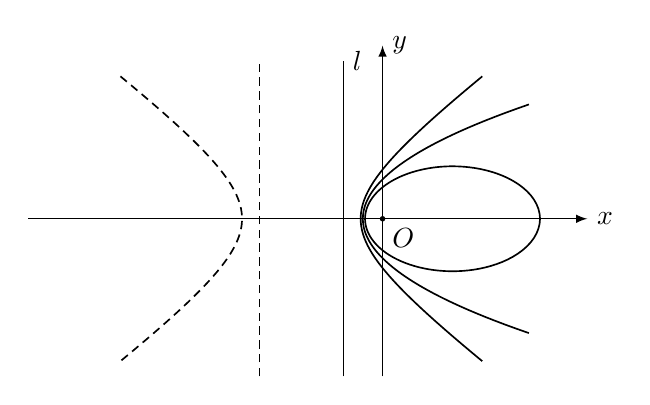
\begin{tikzpicture}[>=latex,scale=1.0]
  \draw [semithick,domain=0:360,samples=200] plot (\x:{0.4/(1-0.8*cos(\x))});
  \draw [semithick,domain=38:322,samples=200] plot (\x:{0.5/(1-cos(\x))});
  \draw [semithick,domain=55:305,samples=200] plot (\x:{0.625/(1-1.25*cos(\x))});
  \begin{scope}[xshift=-2.0625cm]
  \draw [semithick,densely dashed,domain=125:-125,samples=200] plot (\x:{0.625/(1+1.25*cos(\x))});
  \end{scope}
  \draw[->] (-4.5,0)--(2.6,0)node[right]{$x$};
  \draw(-0.5,-2.0)--(-0.5,2.0)node[right]{$l$};
  \draw[densely dashed](-1.5625,-2.0)--(-1.5625,2.0);
  \draw[->] (0,-2.0)--(0,2.2)node[right]{$y$};
  % \node at (38:2.359)[right,green!80!black] {$e=1$};
  % \node at (50:3.180)[right,blue!80!black] {$e>1$};
  % \node at (2,0)[above right,red!80!black] {$e>1$};
  % \node at (0.1,-2.2)[right] {$\rho=\dfrac{ep}{1-e\cos\theta}$};
  \fill (0,0)circle(1pt)node [below right]{$O$};
\end{tikzpicture}
\end{document}